\section{Adaptation d'impédance dans les lignes de transmission --- introduction aux paramètres S}
A ligne sans pertes of impédance caractéristique $Z_C$ closed on a load $Z_L \neq Z_C$
reflects part of the incident power back towards the generator. L'objectif de
l'adaptation d'impédance est de transmettre le maximum de puissance du générateur
vers le récepteur ou l'impédance de charge $Z_L$. It is done by inserting a lossless
reactive network between the line and the load.
The second half of the chapter answers the measurement question that follows: above
a gigahertz the voltages and currents a $Z$ matrix is built from cannot be measured,
so a multipôle is characterised instead by the matrice S, whose entries relate the
ondes de puissance entering the device to the ondes de puissance leaving it.

\begin{notation}
  $Z_C$ is the impédance caractéristique of the line, $Z_G$ the internal impedance of
  the generator, $Z_L$ the load, $Z_E$ the equivalent impedance seen looking into the
  matching network plus the load, and $Z_0$ the impédance de référence of the
  paramètres S. $\beta = 2\pi/\lambda$ is the constante de phase, $\Gamma$ the facteur
  de réflexion, $Y = 1/Z$ an admittance. Unless said otherwise every line in this
  chapter is a ligne sans pertes, so $\beta$ is real and $Z_C$ is real; in practice
  $Z_C = Z_0 = 50\ \Omega$.
\end{notation}

\subsection{Adaptation d'impédances dans les lignes de transmission : introduction}
L'impédance de charge $Z_L$ modélise l'accès du composant ou de la fonction
(amplificateurs, filtres, antennes\dots) suivante intervenant dans une chaîne de
transmission ou une chaîne de réception d'un système de communication. Il est d'autant
plus important d'optimiser et de maximiser ce transfert de puissance utile notamment
pour des systèmes autonomes (smartphones, tablettes, IoT\dots) afin de préserver les
batteries par exemple. Il est donc indispensable d'éviter toutes pertes de puissance
par réflexion due à une désadaptation d'impédance.

Le problème se pose et se résout à deux niveaux : au niveau du générateur et au niveau
de l'impédance de charge. Il faut que, d'une part, le générateur puisse transmettre à
la ligne le maximum de puissance (puissance disponible) et, d'autre part, que le
récepteur reçoive de la ligne le plus possible de cette puissance. \textbf{Dans ce
cours on supposera que le générateur présente une impédance interne adaptée à
l'impédance caractéristique des lignes utilisées}, $Z_G = Z_C$. Only the load end is
therefore ever worked on.

\begin{remark}
  Reflection is not only a loss of efficiency. Lorsqu'une onde est réfléchie, un
  régime d'onde stationnaire existe dans la ligne. La conséquence peut être dans le
  meilleur des cas un système fonctionnant mal et, dans le pire cas, la destruction de
  certains composants du système. It is the voltage maxima of the standing wave that
  destroy them.
\end{remark}

The matching device is a lossless quadripôle, written $Q_{\text{match}}$, inserted
between the line and the load. Un observateur situé à gauche du quadripôle
d'adaptation doit voir une impédance équivalente du système --- quadripôle +
impédance de charge --- égale à l'impédance caractéristique de la ligne, et donc
obtenir un facteur de réflexion, du système quadripôle + impédance de charge, nul.

\begin{figure}[h!]
  \centering
  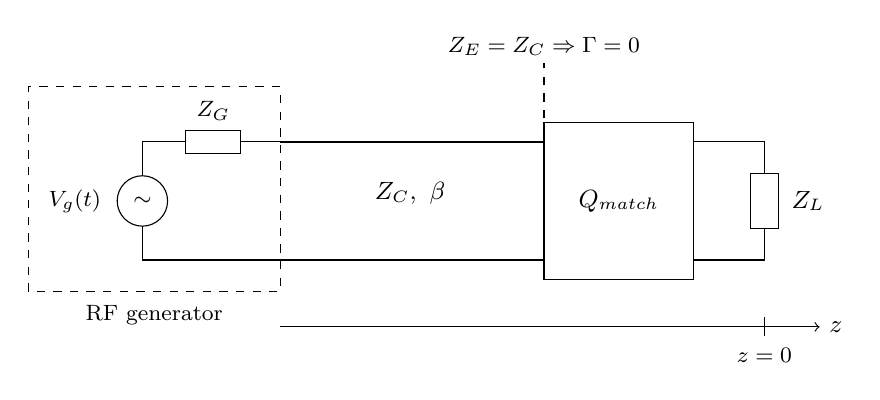
\begin{tikzpicture}[every node/.style={font=\small}]
    % generator
    \draw[dashed] (-1.45,-1.15) rectangle (1.75,1.45);
    \node[font=\footnotesize] at (0.15,-1.45) {RF generator};
    \draw (0,-0.32) -- (0,-0.75) -- (1.75,-0.75);
    \draw (0,0.32) -- (0,0.75) -- (0.55,0.75);
    \draw (0,0) circle (0.32);
    \node[font=\footnotesize] at (0,0) {$\sim$};
    \node[left,font=\footnotesize] at (-0.4,0) {$V_g(t)$};
    \draw (0.55,0.6) rectangle (1.25,0.9);
    \node[above,font=\footnotesize] at (0.9,0.9) {$Z_G$};
    \draw (1.25,0.75) -- (1.75,0.75);
    % line
    \draw[thick] (1.75,0.75) -- (5.1,0.75);
    \draw[thick] (1.75,-0.75) -- (5.1,-0.75);
    \node at (3.4,0.1) {$Z_C,\ \beta$};
    % matching network
    \draw (5.1,-1.0) rectangle (7.0,1.0);
    \node at (6.05,0) {$Q_{\text{match}}$};
    % load
    \draw (7.0,0.75) -- (7.9,0.75) -- (7.9,0.35);
    \draw (7.72,-0.35) rectangle (8.08,0.35);
    \node[right] at (8.12,0) {$Z_L$};
    \draw (7.9,-0.35) -- (7.9,-0.75) -- (7.0,-0.75);
    % axis and reference plane
    \draw[->] (1.75,-1.6) -- (8.6,-1.6) node[right] {$z$};
    \draw (7.9,-1.72) -- (7.9,-1.48);
    \node[below,font=\footnotesize] at (7.9,-1.75) {$z=0$};
    \draw[dashed] (5.1,1.05) -- (5.1,1.75);
    \node[above,font=\footnotesize] at (5.1,1.72) {$Z_E = Z_C \Rightarrow \Gamma = 0$};
  \end{tikzpicture}
  \caption*{Principe de l'adaptation d'impédance. The lossless network
  $Q_{\text{match}}$ turns $Z_L$ into $Z_C$ at its input plane, so nothing is reflected
  back down the line.}
\end{figure}

\begin{prop}[Condition d'adaptation (\textit{matching condition})]
  Written at the generator, the condition reads: adaptation si
  \[Z_C = Z_E^{*},\]
  $Z_E$ étant l'impédance équivalente à $Z_L$ + $Q_{\text{match}}$. Pour une
  ligne sans pertes $Z_C \in \reals$; the condition then reduces to
  \[\boxed{\,Z_E = Z_C\,}\]
  which is the form used everywhere below.
\end{prop}

Afin de limiter les pertes de puissance, il faut de plus que le quadripôle
d'adaptation soit sans pertes afin de ne pas perdre inutilement de la puissance utile.
Pour réaliser cette adaptation d'impédance, on ajoutera des éléments réactifs en série
ou en parallèle, ces éléments étant soit des éléments dits localisés (capacités,
inductances), soit des tronçons de lignes sans pertes. Éléments localisés : composants
réels mais qualité moindre avec les pertes; they are, however, easy to place.
Éléments distribués : réaliser les inductances et capacités avec des tronçons de lignes
(pas de --- ou moins de --- pertes, mais taille !).

\begin{remark}
  En électronique basse fréquence, on utilise aussi le terme d'adaptation
  d'impédance. Un oscilloscope ou un amplificateur, par exemple, possèdent une
  impédance d'entrée très grande pour éviter de diminuer la tension que l'oscilloscope
  doit mesurer ou que l'amplificateur doit amplifier. La source de tension au contraire
  doit posséder une impédance de sortie la plus faible possible. Contrairement à notre
  préoccupation, il ne s'agit pas là d'optimiser le transfert de puissance mais de
  s'arranger pour ne pas écraser la tension disponible.
\end{remark}

\begin{remark}[Warning]
  On ne peut pas adapter une impédance $Z_L$ purement réactive : il faut
  obligatoirement que $Z_L$ possède une partie résistive pour absorber la puissance
  incidente.
\end{remark}

Les dispositifs d'adaptation, que l'on va analyser, sont des dispositifs \textbf{à
bande passante étroite} (\textit{narrowband}) :
\begin{subpart}
  \item l'adaptation en série par une ligne quart d'onde ($\lambda/4$) ou
    transformateur d'impédance ;
  \item l'adaptation en parallèle par l'ajout d'une ligne sans pertes appelée
    \textit{stub} ;
  \item l'adaptation par éléments localisés (quadripôle en « L »).
\end{subpart}

\subsection{Adaptation d'impédance par une ligne quart d'onde ou transformateur d'impédance}
The starting point is the \textit{impédance ramenée} --- the impedance a load presents
after being carried back along a length of line --- established for a ligne sans pertes
as
\[Z(z = -l) = Z_C\,\frac{Z_L + j Z_C \tan(\beta l)}{Z_C + j Z_L \tan(\beta l)}.\]

\begin{prop}[Transformateur d'impédance]
  For $l = \lambda/4$ one has $\beta l = \pi/2$ and $\tan(\beta l) \to \infty$. On
  montre alors que l'impédance
  \[\boxed{\;Z_E = Z\!\left(z = -\lambda/4\right) = \frac{Z'^{\,2}_C}{Z_L}\;}\]
  avec $Z_L$ l'impédance de charge vue sur l'accès opposé de la ligne d'impédance
  caractéristique $Z'_C$, réelle et quelconque. The ligne quart d'onde inverts the load
  about $Z'_C$; this is what makes it a transformateur d'impédance.
\end{prop}

\begin{figure}[h!]
  \centering
  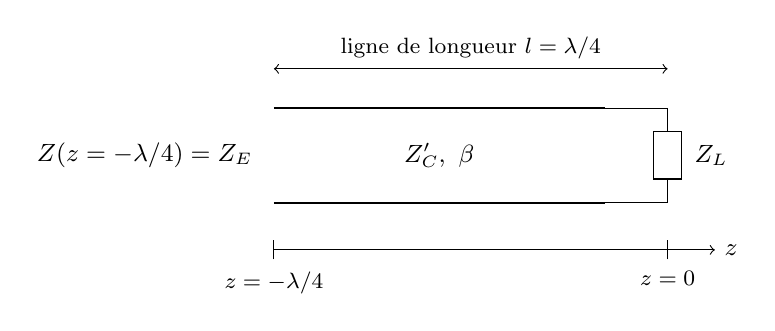
\begin{tikzpicture}[every node/.style={font=\small}]
    \draw[thick] (0,0.6) -- (4.2,0.6);
    \draw[thick] (0,-0.6) -- (4.2,-0.6);
    \node at (2.1,0) {$Z'_C,\ \beta$};
    \draw (4.2,0.6) -- (5.0,0.6) -- (5.0,0.3);
    \draw (4.82,-0.3) rectangle (5.18,0.3);
    \node[right] at (5.22,0) {$Z_L$};
    \draw (5.0,-0.3) -- (5.0,-0.6) -- (4.2,-0.6);
    \draw[<->] (0,1.1) -- (5.0,1.1);
    \node[above,font=\footnotesize] at (2.5,1.1) {ligne de longueur $l = \lambda/4$};
    \draw[->] (0,-1.2) -- (5.6,-1.2) node[right] {$z$};
    \draw (0,-1.32) -- (0,-1.08);
    \draw (5.0,-1.32) -- (5.0,-1.08);
    \node[below,font=\footnotesize] at (0,-1.35) {$z = -\lambda/4$};
    \node[below,font=\footnotesize] at (5.0,-1.35) {$z = 0$};
    \node[left] at (-0.15,0) {$Z(z=-\lambda/4) = Z_E$};
  \end{tikzpicture}
  \caption*{\textit{Impédance ramenée} sur une longueur $l = \lambda/4$.}
\end{figure}

\paragraph{Cas d'une impédance de charge réelle.} On cherche ici à obtenir
$Z_E = Z_C$ où $Z_C$ est l'impédance de référence (exclusivement $50\ \Omega$ dans ce
cours). Setting $Z'^{\,2}_C/Z_L = Z_C$ gives the result to remember: l'adaptation sera
réalisée en utilisant une ligne de longueur $\lambda/4$ d'impédance caractéristique
\[\boxed{\;Z'_C = \sqrt{Z_L Z_C}\;}\]

\begin{remark}[Warning]
  $\lambda$ est la longueur d'onde \emph{dans le matériau} --- tenir compte de la
  permittivité relative $\varepsilon_r$. So $\lambda = c/(f\sqrt{\varepsilon_r})$ and
  the physical length is $l = \lambda/4 = c/(4 f \sqrt{\varepsilon_r})$.
\end{remark}

\paragraph{Cas d'une impédance de charge complexe.} L'impédance caractéristique des
lignes utilisées est réelle afin de ne pas avoir de pertes durant la propagation; a
transformateur d'impédance built from such a line can only invert a real quantity.
Dans ce cas, pour utiliser un transformateur d'impédance, il faut absolument éliminer
la partie imaginaire de l'impédance de charge dans un premier temps :
\begin{subpart}
  \item soit en ajoutant une impédance purement imaginaire (ici $-jX$) pour compenser
    la partie imaginaire --- for a load $Z_L = R + jX$ this leaves $R$ ;
  \item soit en ajoutant un tronçon de ligne d'impédance caractéristique $Z_C$ et de
    longueur $l'$ à ajuster en fonction de la partie imaginaire $jX$ à éliminer ---
    again leaving a real $Z_L = R$ at the plane where the transformateur d'impédance
    starts.
\end{subpart}
Dans les 2 cas, on peut ajouter ensuite la ligne d'impédance caractéristique $Z'_C$ de
longueur $\lambda/4$ pour réaliser l'adaptation finale.

\subsection{Adaptation d'impédance par l'ajout d'un STUB}
\begin{definition}[Stub]
  Un \textit{stub} est un tronçon de ligne sans pertes, associé en parallèle à la ligne
  principale, et terminé par une impédance purement réactive, c'est-à-dire un circuit
  ouvert (CO) ou un court-circuit (CC). Hypothèses : $\beta$ et impédance
  caractéristique identiques à celles de la ligne principale.
\end{definition}

The stub is tapped at the abscissa $z = -d$ and has its own length $d'$. L'adaptation
est obtenue en calculant les longueurs $d$ et $d'$, différentes si on choisit un stub
CC ou un stub CO.

\begin{figure}[h!]
  \centering
  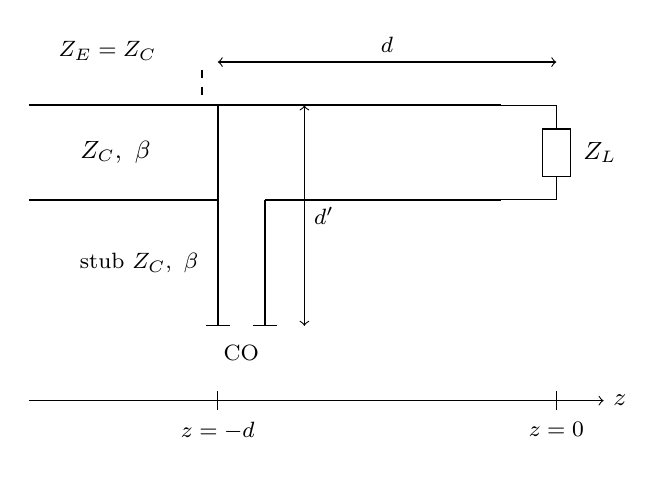
\begin{tikzpicture}[every node/.style={font=\small}]
    % main line
    \draw[thick] (0,0.6) -- (6.0,0.6);
    \draw[thick] (0,-0.6) -- (2.4,-0.6);
    \draw[thick] (3.0,-0.6) -- (6.0,-0.6);
    \node at (1.1,0) {$Z_C,\ \beta$};
    % load
    \draw (6.0,0.6) -- (6.7,0.6) -- (6.7,0.3);
    \draw (6.52,-0.3) rectangle (6.88,0.3);
    \node[right] at (6.92,0) {$Z_L$};
    \draw (6.7,-0.3) -- (6.7,-0.6) -- (6.0,-0.6);
    % stub branch, open-circuited
    \draw[thick] (2.4,0.6) -- (2.4,-2.2);
    \draw[thick] (3.0,-0.6) -- (3.0,-2.2);
    \draw (2.25,-2.2) -- (2.55,-2.2);
    \draw (2.85,-2.2) -- (3.15,-2.2);
    \node[font=\footnotesize] at (2.7,-2.55) {CO};
    \node[font=\footnotesize] at (1.4,-1.4) {stub $Z_C,\ \beta$};
    \draw[<->] (3.5,0.6) -- (3.5,-2.2);
    \node[right,font=\footnotesize] at (3.5,-0.8) {$d'$};
    % distances
    \draw[<->] (2.4,1.15) -- (6.7,1.15);
    \node[above,font=\footnotesize] at (4.55,1.15) {$d$};
    \draw[->] (0,-3.15) -- (7.3,-3.15) node[right] {$z$};
    \draw (2.4,-3.27) -- (2.4,-3.03);
    \draw (6.7,-3.27) -- (6.7,-3.03);
    \node[below,font=\footnotesize] at (2.4,-3.3) {$z = -d$};
    \node[below,font=\footnotesize] at (6.7,-3.3) {$z = 0$};
    \draw[dashed] (2.2,1.05) -- (2.2,0.7);
    \node[above,font=\footnotesize] at (1.0,1.05) {$Z_E = Z_C$};
  \end{tikzpicture}
  \caption*{Conditions d'adaptation par un STUB (ici fermé sur un CO).}
\end{figure}

\begin{prop}[Conditions d'adaptation par un STUB]
  Les conditions d'adaptation sont obtenues lorsque l'impédance globale $Z_E$, formée
  par l'association en \emph{parallèle} de l'impédance $Z_L$ ramenée d'une distance
  $d$ et du stub de longueur $d'$, vérifie $Z_E = Z_C$. Puisque le stub et l'impédance
  de charge ramenée sont en parallèle, on va raisonner en admittance :
  \[\boxed{\;Y_E = Y_C\;}\qquad Y_E = \frac{1}{Z_E},\quad Y_C = \frac{1}{Z_C},\]
  avec
  \[Y_E = \frac{1}{Z_E} = Y_{\text{STUB}} + Y_{Z_L}(z = -d), \qquad
    Y_{Z_L}(z = -d) = \frac{1}{Z(z=-d)}
      = Y_C\,\frac{Z_C + j Z_L \tan(\beta d)}{Z_L + j Z_C \tan(\beta d)}.\]
\end{prop}

En fonction de la terminaison du STUB, on détermine son admittance à partir de
l'expression de l'\textit{impédance ramenée} à l'abscisse $z = -d'$ :
\[
  \text{CO:}\quad Z_{CO} = \infty,\quad
  Y_{\text{STUB}}(z=-d') = \frac{j\tan(\beta d')}{Z_C};
  \qquad
  \text{CC:}\quad Z_{CC} = 0,\quad
  Y_{\text{STUB}}(z=-d') = \frac{1}{j Z_C \tan(\beta d')}.
\]
Equivalently, the stub closed on a circuit ouvert carries back
$Z'_{\text{STUB}} = -jZ_C\cot(\beta d')$.

\begin{remark}
  Each of these three admittances is the reciprocal of the \textit{impédance ramenée}
  $Z(z=-l) = Z_C (Z_L + jZ_C\tan\beta l)/(Z_C + jZ_L\tan\beta l)$ taken over the
  relevant length with the relevant termination (the load, a circuit ouvert or a
  court-circuit), so the tangent's argument is a real electrical length:
  $\tan(\beta d)$ on the load branch, $\tan(\beta d')$ on the stub. The constante de
  phase being real, these tangents are real and contribute no imaginary part of their
  own: on the load branch, for instance, $\tan(\beta d)$ only scales the terms it
  multiplies, and any imaginary part comes from an explicit $j$ or from a complex load.
\end{remark}

\begin{remark}
  Les longueurs $d$ et $d'$ sont déterminées «~modulo~» $\lambda/2$. Il existe donc
  une infinité de solutions, ce qui laisse la possibilité d'éloigner plus ou moins le
  stub de l'impédance de charge. En pratique, on essaie de limiter les longueurs $d$ et
  $d'$ car les lignes ne sont pas parfaites. On peut ainsi jouer sur le choix d'un STUB
  CO ou STUB CC qui permettra de trouver le meilleur compromis. \textbf{Dans ce cours,
  on vous donnera directement la terminaison du STUB pour l'adaptation.}
\end{remark}

\begin{example}[Stub fermé par un circuit ouvert, impédances réelles]
  Les impédances mises en jeu sont réelles. Writing $t = \tan(\beta d)$ and
  rationalising,
  \[Y_{Z_L}(z=-d) = Y_C\,\frac{Z_C Z_L (1+t^2) + j\,t\,(Z_L^2 - Z_C^2)}{Z_L^2 + Z_C^2 t^2},
    \qquad Y_{\text{STUB}} = j Y_C \tan(\beta d').\]
  Setting $Y_E = Y_C$ splits into a real and an imaginary equation. The real part gives
  $Z_C Z_L(1+t^2) = Z_L^2 + Z_C^2 t^2$, i.e.\ $t^2 Z_C(Z_L - Z_C) = Z_L(Z_L - Z_C)$, hence
  \[\boxed{\;\tan(\beta d) = \sqrt{\frac{Z_L}{Z_C}}\;}\]
  Substituting $t^2 = Z_L/Z_C$ into the imaginary part,
  $\tan(\beta d') = -t(Z_L^2-Z_C^2)/(Z_L^2 + Z_C^2 t^2)$, and since
  $Z_L^2 + Z_C^2 t^2 = Z_L(Z_L + Z_C)$,
  \[\boxed{\;\tan(\beta d') = \frac{Z_C - Z_L}{\sqrt{Z_L Z_C}}\;}\]
  Note that $d$ depends only on the ratio $Z_L/Z_C$: the tapping point is the abscissa
  at which the real part of the carried-back admittance is already $Y_C$, and the stub
  then cancels what is left of the susceptance.
\end{example}

\subsection{Adaptation par éléments localisés : quadripôle en « L »}
L'adaptation par éléments localisés consiste à insérer, entre la ligne de propagation
et l'impédance de charge $Z_L$, un quadripôle en forme de « L » constitué de deux
impédances purement imaginaires et matérielles, représentées par $jX_S$ (en série) et
$jX_P$ (en parallèle). Elles sont purement imaginaires afin de ne pas dissiper de
puissance inutilement : l'adaptation se fait avec des impédances qui ne dissipent pas
de puissance afin d'en conserver l'intégralité pour la dissiper dans $Z_L$.

\begin{prop}[Choix de la structure]
  Il y a deux structures possibles. Le choix de la structure dépend de la valeur de la
  partie réelle de l'impédance $Z_L$ à adapter par rapport à $Z_C$ :
  \begin{subpart}
    \item si $Z_L > Z_C$, on mettra en parallèle l'impédance de charge $Z_L$ avec
      l'impédance $jX_P$, le tout sera en série avec $jX_S$, soit
      $Z_E = jX_S + (Z_L \parallel jX_P)$ ;
    \item si $Z_L < Z_C$, on mettra en série l'impédance de charge $Z_L$ avec
      l'impédance $jX_S$, le tout en parallèle avec $jX_P$, soit
      $Z_E = jX_P \parallel (Z_L + jX_S)$.
  \end{subpart}
  Dans les deux cas, l'adaptation est obtenue quand l'impédance globale formée par
  $Z_L$, $jX_S$ et $jX_P$ est égale à $Z_C$.
\end{prop}

\begin{figure}[h!]
  \centering
  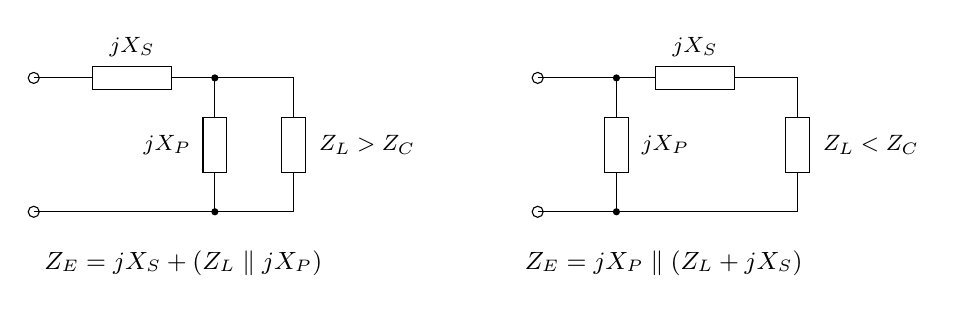
\begin{tikzpicture}[every node/.style={font=\small}]
    % LEFT : ZL > ZC
    \begin{scope}
      \draw (0,1.1) -- (0.75,1.1);
      \draw (0.75,0.95) rectangle (1.75,1.25);
      \node[above,font=\footnotesize] at (1.25,1.25) {$jX_S$};
      \draw (1.75,1.1) -- (3.3,1.1);
      \fill (2.3,1.1) circle (1.3pt);
      \draw (2.3,1.1) -- (2.3,0.6);
      \draw (2.15,-0.1) rectangle (2.45,0.6);
      \node[left,font=\footnotesize] at (2.12,0.25) {$jX_P$};
      \draw (2.3,-0.1) -- (2.3,-0.6);
      \draw (3.3,1.1) -- (3.3,0.6);
      \draw (3.15,-0.1) rectangle (3.45,0.6);
      \node[right,font=\footnotesize] at (3.5,0.25) {$Z_L > Z_C$};
      \draw (3.3,-0.1) -- (3.3,-0.6);
      \draw (0,-0.6) -- (3.3,-0.6);
      \fill (2.3,-0.6) circle (1.3pt);
      \draw (0,1.1) circle (0.07);
      \draw (0,-0.6) circle (0.07);
      \node at (1.9,-1.25) {$Z_E = jX_S + (Z_L \parallel jX_P)$};
    \end{scope}
    % RIGHT : ZL < ZC
    \begin{scope}[xshift=6.4cm]
      \draw (0,1.1) -- (1.5,1.1);
      \draw (1.5,0.95) rectangle (2.5,1.25);
      \node[above,font=\footnotesize] at (2.0,1.25) {$jX_S$};
      \draw (2.5,1.1) -- (3.3,1.1);
      \fill (1.0,1.1) circle (1.3pt);
      \draw (1.0,1.1) -- (1.0,0.6);
      \draw (0.85,-0.1) rectangle (1.15,0.6);
      \node[right,font=\footnotesize] at (1.2,0.25) {$jX_P$};
      \draw (1.0,-0.1) -- (1.0,-0.6);
      \draw (3.3,1.1) -- (3.3,0.6);
      \draw (3.15,-0.1) rectangle (3.45,0.6);
      \node[right,font=\footnotesize] at (3.5,0.25) {$Z_L < Z_C$};
      \draw (3.3,-0.1) -- (3.3,-0.6);
      \draw (0,-0.6) -- (3.3,-0.6);
      \fill (1.0,-0.6) circle (1.3pt);
      \draw (0,1.1) circle (0.07);
      \draw (0,-0.6) circle (0.07);
      \node at (1.6,-1.25) {$Z_E = jX_P \parallel (Z_L + jX_S)$};
    \end{scope}
  \end{tikzpicture}
  \caption*{The two ``L'' structures. Il y a 4 circuits possibles par structure suivant
  le choix des composants pour $jX_S$ et $jX_P$ (inductance-inductance,
  inductance-capacité, capacité-inductance et capacité-capacité). Le choix du type de
  composant se fait en fonction des valeurs réalisables.}
\end{figure}

\begin{example}[$Z_L = 200\ \Omega$ adapté to $Z_e = 50\ \Omega$ at $1\ \mathrm{GHz}$]
  Here $Z_L > Z_e$, so the first structure applies. Il faut débuter par
  $Z_e = jX_S + (Z_L \parallel jX_P)$ et développer la relation précédente. Taking
  $Z_L$ real, the development gives
  \[Z_e = \frac{Z_L X_P^2}{Z_L^2 + X_P^2}
        + j\left(X_S + \frac{Z_L^2 X_P}{Z_L^2 + X_P^2}\right).\]
  Ici $Z_e$ et $Z_L$ sont réelles, alors la partie imaginaire sera nulle. En séparant la
  partie réelle et imaginaire, on obtient alors 2 solutions possibles :
  \[X_P = \mp\, Z_L\sqrt{\frac{Z_e}{Z_L - Z_e}},
    \qquad X_S = \pm\sqrt{Z_e\,(Z_L - Z_e)}.\]
  Numerically, with $Z_L = 200\ \Omega$, $Z_e = 50\ \Omega$ and $F = 1\ \mathrm{GHz}$:
  \begin{center}
    \begin{tabular}{lrrll}
      \toprule
      & $X_P$ & $X_S$ & parallel branch & series branch \\
      \midrule
      Solution 1 & $-115\ \Omega$ & $+86\ \Omega$  & $C = 1.38$ pF & $L = 13.7$ nH \\
      Solution 2 & $+115\ \Omega$ & $-86\ \Omega$  & $L = 18$ nH   & $C = 1.85$ pF \\
      \bottomrule
    \end{tabular}
  \end{center}
  The identification of the component follows the sign of the reactance: une impédance
  imaginaire pure positive $jX = j L \omega$ est une inductance, donc $X = L\omega$ et
  $L = X/(2\pi F)$ ; une impédance imaginaire pure négative est une capacité, soit
  $jX = 1/(jC\omega) = -j/(C\omega)$ donc $X = -1/(C\omega)$ et
  $C = -1/(X\,2\pi F)$.
\end{example}

\begin{remark}
  Over a single denominator, the development above expresses the impédance d'entrée
  $Z_e$ in terms of the load $Z_L$ as
  $Z_e = \left(Z_L X_P^2 + j\left(Z_L^2(X_P + X_S) + X_P^2 X_S\right)\right)/(Z_L^2 + X_P^2)$.
  Since $Z_L$ and the target are both real, it is the bracket multiplying the imaginary
  unit in the numerator that must vanish.
\end{remark}

\begin{example}[$Z_L = 35\ \Omega$ adapté to $Z_e = 50\ \Omega$ at $1\ \mathrm{GHz}$]
  Now $Z_L < Z_e$, so the second structure applies. Il faut débuter par
  $Z_e = jX_P \parallel (Z_L + jX_S)$ ; en développant la relation précédente, on
  obtient
  \[Z_e = \frac{Z_L X_P^2}{Z_L^2 + (X_P + X_S)^2}
        + j\,\frac{X_P Z_L^2 + X_P X_S (X_P + X_S)}{Z_L^2 + (X_P + X_S)^2}.\]
  La partie imaginaire sera nulle ; on obtient alors 2 solutions possibles, with the
  roles of $Z_e$ and $Z_L$ exchanged relative to the previous case:
  \[X_P = \mp\, Z_e\sqrt{\frac{Z_L}{Z_e - Z_L}},
    \qquad X_S = \pm\sqrt{Z_L\,(Z_e - Z_L)}.\]
  \begin{center}
    \begin{tabular}{lrrll}
      \toprule
      & $X_P$ & $X_S$ & parallel branch & series branch \\
      \midrule
      Solution 1 & $-76\ \Omega$ & $+23\ \Omega$ & $C = 2.09$ pF  & $L = 3.66$ nH \\
      Solution 2 & $+76\ \Omega$ & $-23\ \Omega$ & $L = 12.1$ nH  & $C = 6.92$ pF \\
      \bottomrule
    \end{tabular}
  \end{center}
\end{example}

\begin{remark}
  The eight component values in the two tables follow from $L = X_S/(2\pi F)$ and
  $C = -1/(X_S\,2\pi F)$ at $F = 1\ \mathrm{GHz}$, and likewise for the parallel
  branch, applied to the rounded reactances of the tables. That rounding limits their
  precision: for the series inductance $L = 13.7$ nH of the first table,
  $X_S/(2\pi F)$ gives $13.69$ nH with the rounded $X_S = 86\ \Omega$, and $13.78$ nH
  with the unrounded $X_S = \sqrt{7500} = 86.6\ \Omega$.
\end{remark}

\begin{conclusion}
  The three devices answer the same equation $Z_E = Z_C$ with different hardware. The
  $\lambda/4$ transformateur d'impédance needs a real load and a line whose impédance
  caractéristique is a free design parameter; the stub needs only lines identical to
  the main one but two lengths to tune; the ``L'' network needs two reactive
  components and no line at all, at the cost of real components that have losses,
  where line sections have fewer losses but cost size. All three are à bande passante
  étroite, since each relies on a reactance or an electrical length that is correct at
  one frequency only.
\end{conclusion}

\subsection{Introduction aux paramètres S}
\subsubsection{La matrice Z en hyperfréquence}
Un \textbf{quadripôle} (\textit{two-port}) est un dispositif à 2 accès qui modélise le
transfert des grandeurs électriques, tension $V$ et courant $i$, au niveau de chaque
accès. Un \textbf{accès} (\textit{access}) est défini par 2 conducteurs simples séparés
par un diélectrique (par exemple une ligne de transmission) ; il est appelé
\textbf{dipôle} (\textit{one-port}). Un quadripôle est entièrement caractérisé par sa
matrice $Z$,
\[\begin{pmatrix} V_1 \\ V_2 \end{pmatrix}
  = Z \begin{pmatrix} i_1 \\ i_2 \end{pmatrix},
  \qquad
  \begin{cases} V_1 = Z_{11} i_1 + Z_{12} i_2 \\ V_2 = Z_{21} i_1 + Z_{22} i_2 \end{cases}\]
whose entries are obtained one at a time by opening one accès. For instance
\[Z_{11} = \left.\frac{V_1}{i_1}\right|_{i_2 = 0},\]
mesuré en fermant l'accès 2 sur un circuit ouvert ($i_2 = 0$), en connectant une
source de courant à l'accès 1 et en mesurant la tension $V_1$. For a T-shaped
resistive attenuator of arms $R_1, R_2, R_3$ this gives $Z_{11} = R_1 + R_2$,
$Z_{12} = Z_{21} = R_2$, $Z_{22} = R_2 + R_3$.

\begin{remark}[Measurement at hyperfréquences]
  Dans le cadre des fréquences très élevées (> GHz) : \textbf{hyperfréquences}
  (\textit{microwave}), microondes, mmW. There this procedure breaks down on three
  counts:
  \begin{subpart}
    \item les court-circuits et circuits ouverts sont difficiles à réaliser sur une
      large bande de fréquences, because the longueur d'onde becomes comparable with
      the dimensions of the lines and components, so the \textit{impédance ramenée} of
      a nominal short is not a short at the plane of interest;
    \item la mesure de la tension est complexe voire impossible (nécessite des ADCs
      ultra rapides) ;
    \item la réalisation des sources de courant est ardue.
  \end{subpart}
  La seule grandeur facilement mesurable en hyperfréquence est la \textbf{puissance}.
  La matrice $Z$ est très pratique mais très difficile à utiliser pour des fréquences
  très élevées.
\end{remark}

La \textbf{matrice S} (\textit{scattering matrix}) est un outil essentiel de
caractérisation de multipôles (dispositifs à $N$ accès) en hyperfréquence. Les facteurs de cette matrice, appelés \textbf{paramètres
S} (\textit{scattering parameter}), lient les puissances entrantes dans un multipôle
aux puissances sortantes, et sont basés uniquement sur des mesures de puissance. The
motivation is not academic: les puissances mises en jeu dans la majorité des
applications en hyperfréquence sont très faibles (pour la 5G, le seuil de détection
est fixé à une puissance de réception de $-102\ \mathrm{dBm}$, soit environ
$10^{-10}\ \mathrm{mW}$ ou $10^{-13}\ \mathrm{W}$). Connaître la distribution de la
puissance utile dans un dispositif est donc incontournable si on veut optimiser le
fonctionnement afin de limiter la consommation électrique et donc naturellement
prolonger l'autonomie des dispositifs sans fil.

\subsubsection{Notion d'onde de puissance}
Un multipôle linéaire à $N$ accès possède $2N$ pôles. On choisira une
\textbf{impédance de référence} (\textit{reference impedance}) des paramètres S,
réelle, que l'on notera $Z_0$. It is fixed once and for all. On note les tensions
incidentes $V_k^{+}$ et les courants incidents $I_k^{+}$ associés, dans le plan de
référence de l'accès $k$ ($k = 1 \dots N$), ainsi que les tensions réfléchies $V_k^{-}$
et les courants réfléchis $I_k^{-}$ associés. On écrit alors la tension totale et le
courant total à l'accès $k$ :
\[V_k = V_k^{+} + V_k^{-},
  \qquad I_k = I_k^{+} + I_k^{-} = \frac{1}{Z_0}\left(V_k^{+} - V_k^{-}\right),\]
equivalently $V_k^{+} = \tfrac{1}{2}(V_k + Z_0 I_k)$ and
$V_k^{-} = \tfrac{1}{2}(V_k - Z_0 I_k)$.

\begin{remark}
  The current relation is written here with the minus sign, as above: the incident and
  reflected currents are both counted along a single reference direction, towards the
  load, so the reflected current enters the total current with a minus sign. Another
  convention writes «~$V^{+} = Z_0 I^{+}$ et $V^{-} = Z_0 I^{-}$~», drawing
  $I^{-}$ as an arrow pointing back towards the source, i.e.\ $I^{-}$ taken as a
  magnitude along the reverse direction. The two conventions differ only in that
  reference direction for the reflected current: both give $\Gamma = V^{-}/V^{+}$ and
  the same power expressions below. These notes use the single reference direction
  throughout.
\end{remark}

La puissance des ondes incidentes ($P_k^{+}$) et réfléchies ($P_k^{-}$) sur l'accès $k$
s'exprime comme
\[P_k^{+} = \frac{1}{2}\Re\!\left(V_k^{+} I_k^{+*}\right)
          = \frac{1}{2}\Re\!\left(\frac{V_k^{+} V_k^{+*}}{Z_0}\right)
          = \frac{\left|V_k^{+}\right|^2}{2 Z_0},
  \qquad
  P_k^{-} = \frac{\left|V_k^{-}\right|^2}{2 Z_0}.\]
On pourrait caractériser le multipôle en reliant les puissances $P_k^{+}$ et $P_k^{-}$,
mais la phase des tensions et des courants disparaît --- mesure scalaire (perte de
l'information de la phase). On préfère donc définir des \textbf{ondes de puissance}
(\textit{power wave}) $a_k$ (entrantes) et $b_k$ (sortantes) :

\begin{definition}[Ondes de puissance]
  \[\boxed{\;
    a_k = \frac{V_k + Z_0 I_k}{2\sqrt{Z_0}} = \frac{V_k^{+}}{\sqrt{Z_0}},
    \qquad
    b_k = \frac{V_k - Z_0 I_k}{2\sqrt{Z_0}} = \frac{V_k^{-}}{\sqrt{Z_0}},
    \qquad k = 1 \dots N,\;}\]
  avec $Z_0$ l'impédance de référence. They carry the powers
  \[P^{+} = \frac{1}{2}\left|a\right|^2, \qquad P^{-} = \frac{1}{2}\left|b\right|^2.\]
\end{definition}

\begin{remark}
  Les ondes de puissance $a$ et $b$ dépendent de $V$ et $I$, qui sont définies par
  l'équation des télégraphistes et sont des grandeurs complexes (module et phase). Il
  est donc important de connaître \emph{l'endroit} où on mesure $a$ et $b$, car la
  phase associée sera affectée si le plan de mesure n'est pas fixé.
\end{remark}

\subsubsection{Définition de la matrice S}
\begin{definition}[Matrice S]
  On appelle \textit{matrice S} la matrice qui lie, dans un multipôle, le vecteur ondes
  entrantes $(a)$ au vecteur ondes sortantes $(b)$. Ceci s'exprime de la manière
  suivante :
  \[(b) = S\,(a), \qquad
  \begin{pmatrix} b_1 \\ b_2 \\ \vdots \\ b_{N-1} \\ b_N \end{pmatrix}
  =
  \begin{pmatrix}
    S_{11}    & S_{12}    & \dots & S_{1N} \\
    S_{21}    & S_{22}    & \dots & S_{2N} \\
    \vdots    & \vdots    & \ddots& \vdots \\
    S_{N-1\,1}& S_{N-1\,2}& \dots & S_{N-1\,N} \\
    S_{N1}    & S_{N2}    & \dots & S_{NN}
  \end{pmatrix}
  \begin{pmatrix} a_1 \\ a_2 \\ \vdots \\ a_{N-1} \\ a_N \end{pmatrix},\]
  soit $b_k = S_{k1} a_1 + S_{k2} a_2 + \dots + S_{kN} a_N$ pour chaque $k$. La matrice
  S permet donc de calculer les ondes sortantes $b_k$ d'un accès $k$ connaissant les
  ondes $a$ à tous les accès du multipôle.
\end{definition}

\begin{remark}[Properties to remember]
  \begin{subpart}
    \item La matrice S caractérise un multipôle \emph{linéaire} en régime
      \emph{harmonique}.
    \item Les paramètres S sont des nombres complexes.
    \item Les paramètres S dépendent généralement de la fréquence.
    \item Les paramètres S dépendent du plan de référence choisi et de l'impédance de
      référence $Z_0$. La plupart du temps, on utilise une impédance de référence $Z_0$
      égale à l'impédance caractéristique des lignes $Z_C$, qui sera généralement
      $50\ \Omega$, afin d'uniformiser sur une valeur internationale commune.
  \end{subpart}
\end{remark}

\subsubsection{Cas du dipôle}
Dans le cas d'un dipôle (une antenne par exemple), on a un seul accès et 2 ondes $a_1$
et $b_1$. On a alors $b_1 = S_{11} a_1$, soit
\[\boxed{\;S_{11} = \frac{b_1}{a_1} = \frac{V_1^{-}}{V_1^{+}} = \Gamma_1\;}\]
qui est donc le facteur de réflexion à l'accès du dipôle. A dipôle carries reflection
information and nothing else.

\subsubsection{Cas du quadripôle}
Dans le cas d'un quadripôle, les ondes entrante et sortante sont reliées par la
relation
\[\begin{cases} b_1 = S_{11} a_1 + S_{12} a_2 \\ b_2 = S_{21} a_1 + S_{22} a_2. \end{cases}\]
Afin de déterminer chaque paramètre S, il faut alimenter le quadripôle par l'accès 1 et
fermer l'accès 2 par une impédance de charge adaptée (c'est-à-dire l'impédance de
référence $Z_0$). L'onde $a_2$ est donc par définition nulle puisqu'il n'y a pas de
réflexion sur l'impédance de charge qui est adaptée. On a alors $b_1 = S_{11} a_1$,
$b_2 = S_{21} a_1$, et on obtient
\[\boxed{\;
  \begin{cases}
    S_{11} = \dfrac{b_1}{a_1} = \Gamma_1 \\[2ex]
    S_{21} = \dfrac{b_2}{a_1} = Tr_{21}
  \end{cases}
  \quad \text{for } a_2 = 0.\;}\]

\begin{remark}
  Ceci n'est valable \emph{que} si $a_2$ est nulle ! Forgetting the termination is the
  classical error: with $a_2 \neq 0$ the ratio $b_1/a_1$ is not $S_{11}$.
\end{remark}

$S_{11}$ est donc le facteur de réflexion $\Gamma_1$ sur l'accès 1 quand aucune onde ne
rentre par l'autre accès, c'est-à-dire lorsqu'aucune cause extérieure au quadripôle
n'est responsable d'un retour d'onde. $S_{21}$ est le \textbf{facteur de transmission
direct} (\textit{direct transmission factor}) $Tr_{21}$, c'est-à-dire de l'accès 1 vers
l'accès 2, lorsqu'aucune onde ne rentre par l'accès 2, c'est-à-dire «~qu'aucun obstacle
extérieur ne vient diminuer l'onde transmise~».

Pour obtenir $S_{12}$ et $S_{22}$, on procède de manière symétrique : il faut alimenter
le quadripôle par l'accès 2 et fermer l'accès 1 par une impédance de charge adaptée ;
dans ce cas $a_1 = 0$ et
\[\boxed{\;
  \begin{cases}
    S_{12} = \dfrac{b_1}{a_2} = Tr_{12} \\[2ex]
    S_{22} = \dfrac{b_2}{a_2} = \Gamma_2
  \end{cases}
  \quad \text{for } a_1 = 0,\;}\]
$S_{22}$ étant le facteur de réflexion $\Gamma_2$ sur l'accès 2 et $S_{12}$ le
\textbf{facteur de transmission inverse} (\textit{reverse transmission factor}),
c'est-à-dire de l'accès 2 vers l'accès 1.

\begin{figure}[h!]
  \centering
  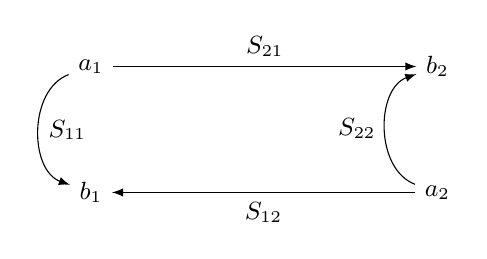
\begin{tikzpicture}[>=latex,every node/.style={font=\small}]
    \node (a1) at (0,1.6) {$a_1$};
    \node (b2) at (4.4,1.6) {$b_2$};
    \node (b1) at (0,0) {$b_1$};
    \node (a2) at (4.4,0) {$a_2$};
    \draw[->] (a1) -- node[above] {$S_{21}$} (b2);
    \draw[->] (a2) -- node[below] {$S_{12}$} (b1);
    \draw[->] (a1) to[bend right=70] node[right,pos=0.5] {$S_{11}$} (b1);
    \draw[->] (a2) to[bend left=70] node[left,pos=0.5] {$S_{22}$} (b2);
  \end{tikzpicture}
  \caption*{The \textbf{graphe de fluence} (\textit{signal-flow graph}) of a
  quadripôle.}
\end{figure}

\begin{prop}[Quelques caractéristiques]
  Un quadripôle est
  \begin{subpart}
    \item \textbf{adapté} si $S_{ii} = 0$ ;
    \item \textbf{réciproque} (\textit{reciprocal}) si $S_{ij} = S_{ji}$ ;
    \item \textbf{symétrique} (\textit{symmetric}) si $S_{ii} = S_{jj}$ \emph{et}
      $S_{ij} = S_{ji}$ ;
    \item \textbf{passif} (\textit{passive}) si tous les paramètres S vérifient
      $|S| \le 1$ ;
    \item \textbf{actif} (\textit{active}) si au moins un des paramètres S est
      supérieur à $1$.
  \end{subpart}
\end{prop}

\subsubsection{Mesure des paramètres S}
Pour caractériser un multipôle par ses paramètres S, il faut alimenter, par un
générateur avec une impédance interne adaptée, l'un des accès qui servira de référence
et fermer les autres accès par une impédance de charge adaptée. Sweeping which accès is
fed and which are terminated fills the matrix column by column. En pratique on réalise
la mesure à l'aide d'un analyseur de réseaux vectoriel (VNA), which is vectorial
precisely because it recovers the phase of $a$ and $b$ that a scalar wattmètre would
throw away.

\subsection{Adaptation d'impédance et paramètres S}
This example chains everything in the chapter: the measured $S_{11}$ of an antenne is
read as a facteur de réflexion, converted into an impedance, modelled by éléments
localisés, cancelled by a parallel reactance and finally transformed by a $\lambda/4$
line.

\begin{figure}[h!]
  \centering
  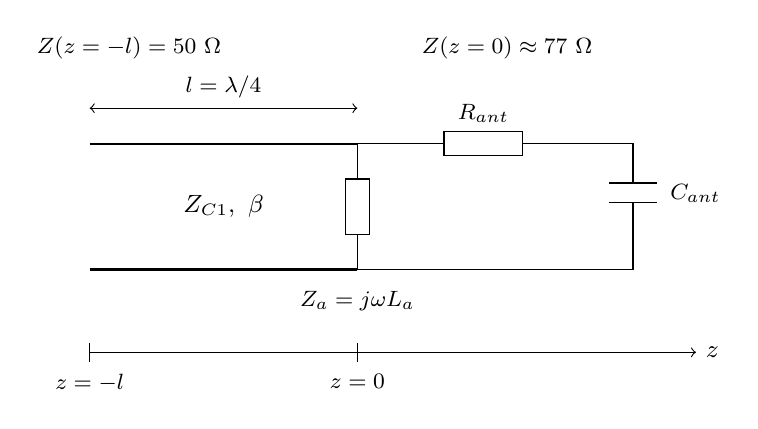
\begin{tikzpicture}[every node/.style={font=\small}]
    % quarter-wave line
    \draw[thick] (0,0.8) -- (3.4,0.8);
    \draw[thick] (0,-0.8) -- (3.4,-0.8);
    \node at (1.7,0) {$Z_{C1},\ \beta$};
    \draw[<->] (0,1.25) -- (3.4,1.25);
    \node[above,font=\footnotesize] at (1.7,1.25) {$l = \lambda/4$};
    % shunt inductance at z = 0
    \draw (3.4,0.8) -- (3.4,0.35);
    \draw (3.25,-0.35) rectangle (3.55,0.35);
    \draw (3.4,-0.35) -- (3.4,-0.8);
    \node[font=\footnotesize] at (3.4,-1.2) {$Z_a = j\omega L_a$};
    % antenna model
    \draw (3.4,0.8) -- (4.5,0.8);
    \draw (3.4,-0.8) -- (6.9,-0.8);
    \draw (4.5,0.65) rectangle (5.5,0.95);
    \node[above,font=\footnotesize] at (5.0,0.95) {$R_{ant}$};
    \draw (5.5,0.8) -- (6.9,0.8) -- (6.9,0.3);
    \draw (6.6,0.3) -- (7.2,0.3);
    \draw (6.6,0.05) -- (7.2,0.05);
    \node[right,font=\footnotesize] at (7.25,0.17) {$C_{ant}$};
    \draw (6.9,0.05) -- (6.9,-0.8);
    % axis
    \draw[->] (0,-1.85) -- (7.7,-1.85) node[right] {$z$};
    \draw (0,-1.97) -- (0,-1.73);
    \draw (3.4,-1.97) -- (3.4,-1.73);
    \node[below,font=\footnotesize] at (0,-2.0) {$z = -l$};
    \node[below,font=\footnotesize] at (3.4,-2.0) {$z = 0$};
    \node[above,font=\footnotesize] at (0.5,1.75) {$Z(z=-l) = 50\ \Omega$};
    \node[above,font=\footnotesize] at (5.3,1.75) {$Z(z=0) \approx 77\ \Omega$};
  \end{tikzpicture}
  \caption*{The quadripôle d'adaptation $Q$: the parallel inductance $L_a$ makes $Z(z=0)$
  real, and the $\lambda/4$ section of impedance $Z_{C1}$ then transforms
  $77\ \Omega$ into $50\ \Omega$. La longueur entre $Z_{ant}$ et l'accès en sortie du
  quadripôle $Q$ est nulle.}
\end{figure}

\begin{example}[Antenne à $1\ \mathrm{GHz}$, $S_{11} = 0.3\,e^{-j60^{\circ}}$, $Z_0 = 50\ \Omega$]
  \textbf{L'antenne est-elle adaptée ?} Le module $|S_{11}| = 0.3 \neq 0$. L'antenne
  n'est donc pas adaptée et une partie de la puissance sera perdue par réflexion.

  \medskip
  \textbf{Impédance d'entrée.} L'antenne est un dispositif à un seul accès, on peut
  donc dire que $\Gamma_{ant} = S_{11}$ avec comme impédance de référence
  $Z_0 = 50\ \Omega$, et
  \[\Gamma_{ant} = S_{11} = \frac{Z_{ant} - Z_0}{Z_{ant} + Z_0}
    \quad\Longrightarrow\quad
    Z_{ant} = Z_0\,\frac{1 + S_{11}}{1 - S_{11}}.\]
  Avec $S_{11} = 0.3\,e^{-j60^{\circ}} = 0.15 - j\,0.26$, on obtient alors
  \[Z_{ant} = R_{ant} + j X_{ant} = 58 - j\,32.9\ \Omega.\]
  La réactance en série est négative, ce qui signifie ici que le composant est une
  capacité, $X_{ant} = -1/(C_{ant}\omega)$, d'où
  \[C_{ant} = \frac{1}{32.9 \times 2\pi \times 10^{9}} = 4.83\ \mathrm{pF}.\]
  Par conséquent l'antenne est modélisée par une résistance $R_{ant} = 58\ \Omega$ en
  série avec une capacité $C_{ant} = 4.83\ \mathrm{pF}$ pour une fréquence de
  fonctionnement fixée à $1\ \mathrm{GHz}$.

  \medskip
  \textbf{Pourquoi il faut ajouter une réactance $Z_a$.} Cette réactance va permettre
  d'annuler la partie imaginaire de $Z_{ant}$ : l'impédance
  $Z(z=0) = Z_{ant} \parallel Z_a$ sera donc réelle, ce qui est obligatoire pour
  réaliser une adaptation par transformateur d'impédance réalisé grâce à une ligne sans
  pertes de longueur $\lambda/4$. Pour éliminer l'effet capacitif de l'antenne, on doit
  donc connecter en parallèle un élément inductif, $Z_a = jX = j\omega L_a$.
  L'admittance formée par l'association en parallèle est égale à
  \[Y(z=0) = Y_{ant} + Y_a
    = \frac{1}{R_{ant} + 1/(j\omega C_{ant})} + \frac{1}{j\omega L_a}
    = \frac{1}{1 + \omega^2 R_{ant}^2 C_{ant}^2}
      \left(\omega^2 R_{ant} C_{ant}^2
        + j\,\frac{L_a C_{ant}\omega^2 - 1}{\omega L_a}\right).\]
  On doit annuler la partie imaginaire, c'est-à-dire que $L_a C_{ant}\omega^2 = 1$,
  soit
  \[L_a = \frac{1}{C_{ant}\,\omega^2} = 5.24\ \mathrm{nH}.\]

  \medskip
  \textbf{Le transformateur d'impédance $\lambda/4$.} Après l'ajout de cette
  inductance, l'admittance $Y(z=0)$ sera purement réelle et
  \[Z(z=0) = \frac{1}{Y(z=0)}
    = \frac{1 + \omega^2 R_{ant}^2 C_{ant}^2}{\omega^2 R_{ant} C_{ant}^2}
    \approx 77\ \Omega.\]
  Le tronçon de ligne ajouté, sans pertes, de longueur $l = \lambda/4$, aura une
  impédance caractéristique choisie de telle sorte que l'impédance ramenée soit
  $Z(z=-l) = Z_{C1}^2/Z(z=0) = 50\ \Omega$, d'où
  \[\begin{cases}
      Z_{C1} = \sqrt{Z(z=0)\,Z(z=-l)} = \sqrt{77 \times 50} = 62\ \Omega \\[1ex]
      l = \dfrac{\lambda}{4} = \dfrac{c}{4 f \sqrt{\varepsilon_r}} = 7.5\ \mathrm{cm}
    \end{cases}\]
  pour une permittivité relative $\varepsilon_r = 1$ de la ligne ajoutée. The complete
  quadripôle d'adaptation $Q$ is thus a $5.24\ \mathrm{nH}$ inductance in parallel at
  $z = 0$, followed by $7.5\ \mathrm{cm}$ of $62\ \Omega$ line.
\end{example}

\begin{remark}
  L'impédance d'entrée de l'antenne est modélisée par une résistance $R_{ant}$ et une
  réactance $jX_{ant}$ placées en série à l'abscisse $z = 0$ ; ceci est un modèle où les
  longueurs de ligne entre elles et le plan d'accès sont nulles. That idealisation is
  what makes $Z_{ant} = Z_0(1+S_{11})/(1-S_{11})$ directly usable: as soon as a length of line
  sits between the components and the reference plane, the phase of $S_{11}$ --- and
  with it the extracted $R$ and $X$ --- changes, which is the «~les paramètres S
  dépendent du plan de référence choisi~» caveat made concrete.
\end{remark}
